\documentclass[14pt]{extarticle}
\usepackage{amsfonts, amsmath}
\usepackage{graphicx, wrapfig}
\graphicspath{ {./images/} }
\usepackage[margin=0.75in]{geometry}

\newcommand\setIndent[1]{\setlength\itemindent{#1}}

\newenvironment{indentone}{\begin{adjustwidth}{2em}{0em}}{\end{adjustwidth}}

\newcommand\Reals{{\mathbb{R}}}
\newcommand{\eone}{\epsilon_1}
\newcommand{\etwo}{\epsilon_2}


\begin{document}
	\begin{center}
		\textbf{\Large Topological Data Analysis in Markets}
	\end{center}
	\begin{center}
		Shayan Salesi
	\end{center}

\part{An introduction}
	
\section*{1.1 The Ludic Fallacy}
	
The rise of algorithmic trading has changed the financial landscape 
from boiler rooms and bucket shops - places people used to buy
physical stock certificates - to the electric bindings of co-located
data servers. With the exponential output of statistical methods in the twentieth-century, especially those pertaining to time-series data, the financial markets became increasingly gameified, in the sense that poker is a "game." Thus began the rapid deployment of smoothing techniques (moving averages), derived indicators (oscillators), bar patterns, and momentum indicators (RSI). \\

At the same time, the human tendency to appeal to platonic pareidolia began to affect actors in the market, and came the advent of drawing resistance and support lines in stock charts, and looking for repeatable patterns. But this has given birth to an inverted system, in which we study the market as an object in itself, instead of studying the participants within the market. As a result, the primary method of financial data analysis is time-series analysis, as the assumption is that the market is an object in and of itself moving through time. \\

And so we have standardized the idea of the invisible hand, and lost sight of the truth: there is no market, only participants. Alas, man has again gameified another non-game system.
	
\section*{1.2 Financial Jargon}
We first orient the reader with some concepts in financial data. \\

A stock is a certificate of ownership within a company. For example I can create a company and issue 100 shares, and giving myself 50 of them, I now own 50 of my company. After the first issue of stock, called the initial offering, the stocks enter into the secondary market, known as stock exchanges. Here, they are continuously auctioned from 9:30-4pm. A stock quote would look like Table 1 above. In it, the most important fields are the bid and the ask; the bid is how much the highest buyer is willing to pay for this stock, and the ask is how much the lowest seller is willing to sell for. \\
% stock quote picture
\begin{table}%[h!]
\centering
\caption{Micron Technology Inc.}
 \begin{tabular}{||c c c c c c c||}
 \hline
 Last Trade & Time & Change & Prev Close & Open & Bid & Ask \\ [0.5ex] 
 \hline\hline
 50.2 & 01/02/2020,07:01:11.656 & +0.27 & 49.93 & 50.12 & 50.22 & 50.23 \\ [1ex] 
 \hline
 \end{tabular}
\end{table}

When a trader enters a trade into the market, there are two primary order types: the market order, and the limit order. The market order will execute at the nearest best bid or offer - if the trader wants to buy Micron, it will execute at the asking price, and if they want to sell at market, it will execute at the bid. In effect, market orders are paying a premium of the spread between the bid and the ask, because they are taking away liquidity from the market (explained further after limit orders). Limit orders are when the trader specifies their trading price: for example, I want to buy Micron at 50.15, so I put a limit order for 50.15. That order sits there until the market price (bid/ask) trade down to that price. In this case, I am providing liquidity to the market, as I am offering traders that put in market orders the opportunity to have their order executed promptly. I pay no bid/ask spread premium when executing a limit order.\\

\begin{figure}[h]
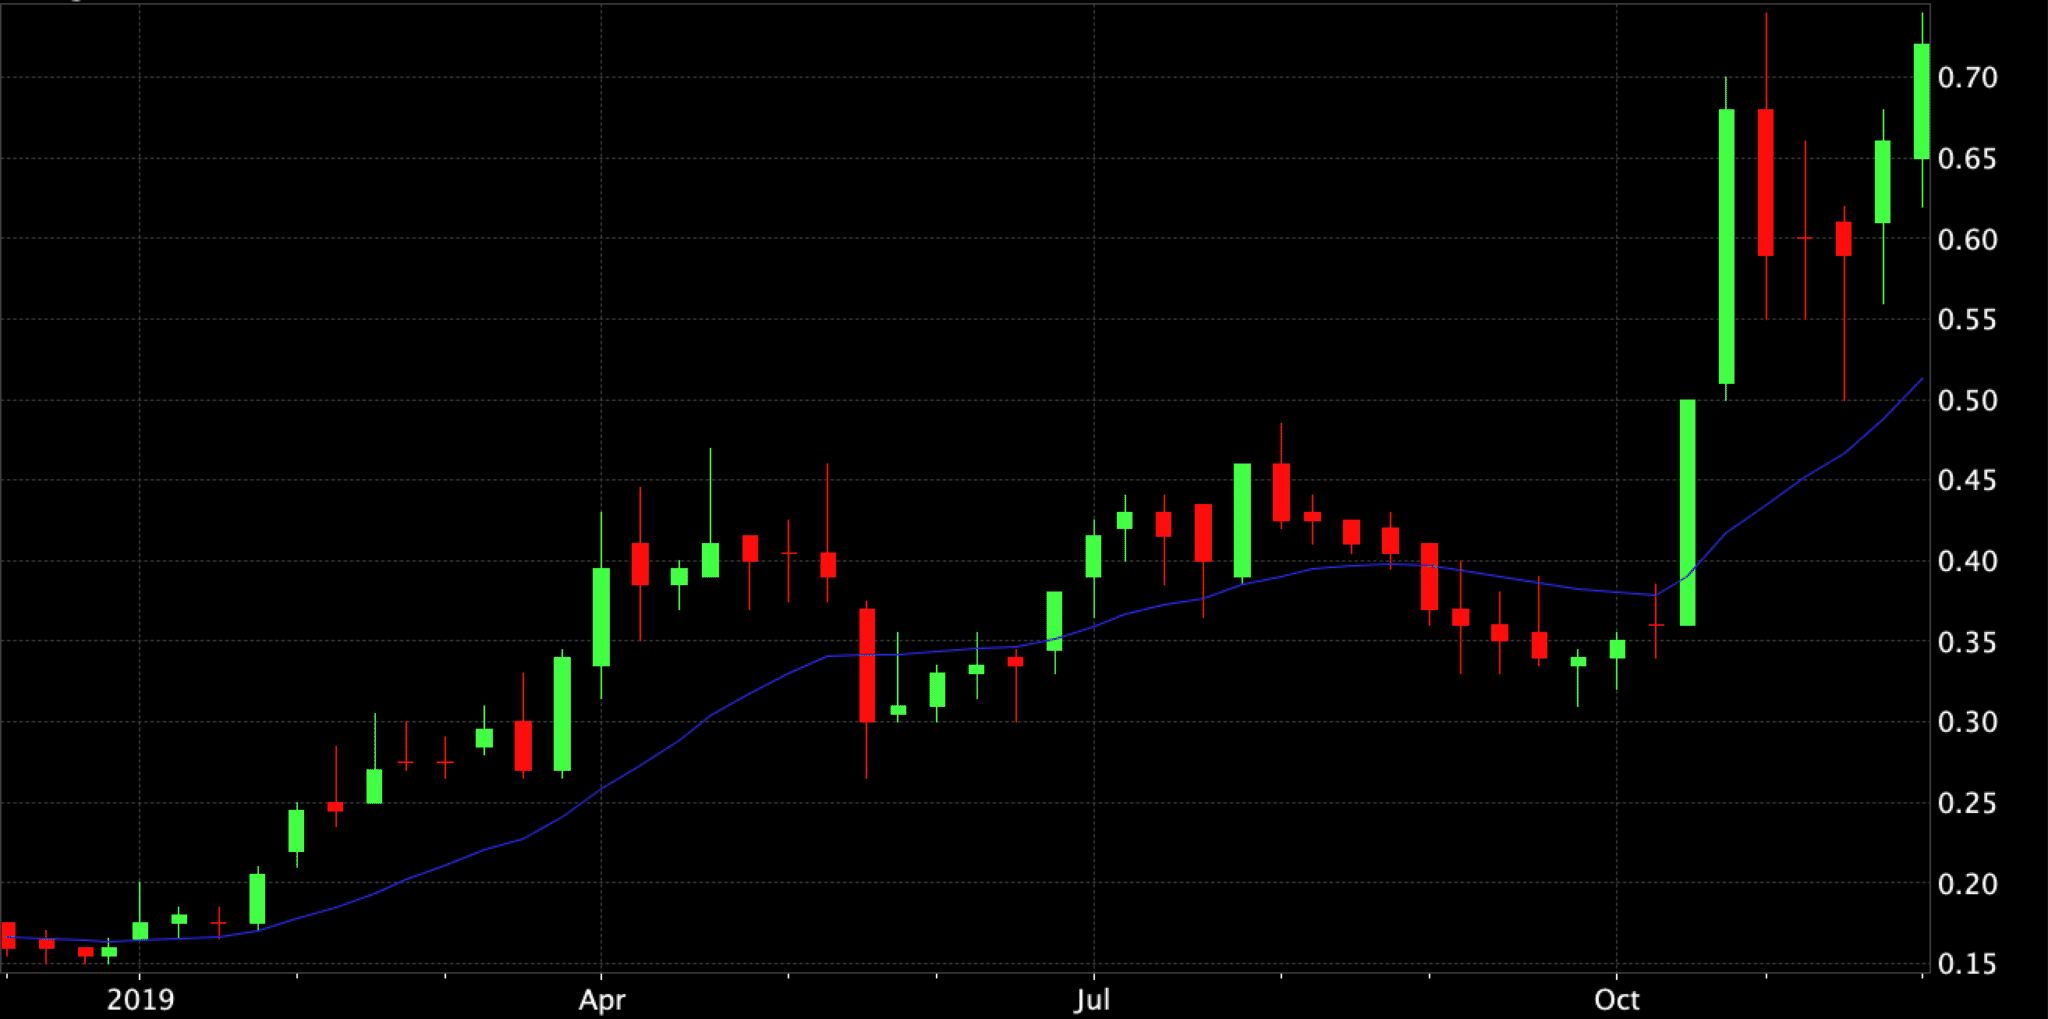
\includegraphics[scale=0.1]{stock_chart}
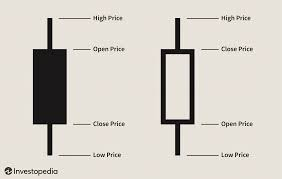
\includegraphics[scale=0.6]{candlestick}
\centering
\end{figure}

Data can be represented in many ways, but the usual flavour is candlestick data. An example can be seen in the images above. Candlestick data has a timestamp, and a time frame. A five minute candle would include the open, high, low, close of the previous five minutes. Most of technical analysis of stock markets is carried out using the OHLC (open high low close) data type; indicators are built on top of this data. For example in the following graphic, we see a candlestick chart.
\newpage

\begin{wrapfigure}{r}{0.4\linewidth}
%\centering
%\rule{0.9\linewidth}{0.75\linewidth}
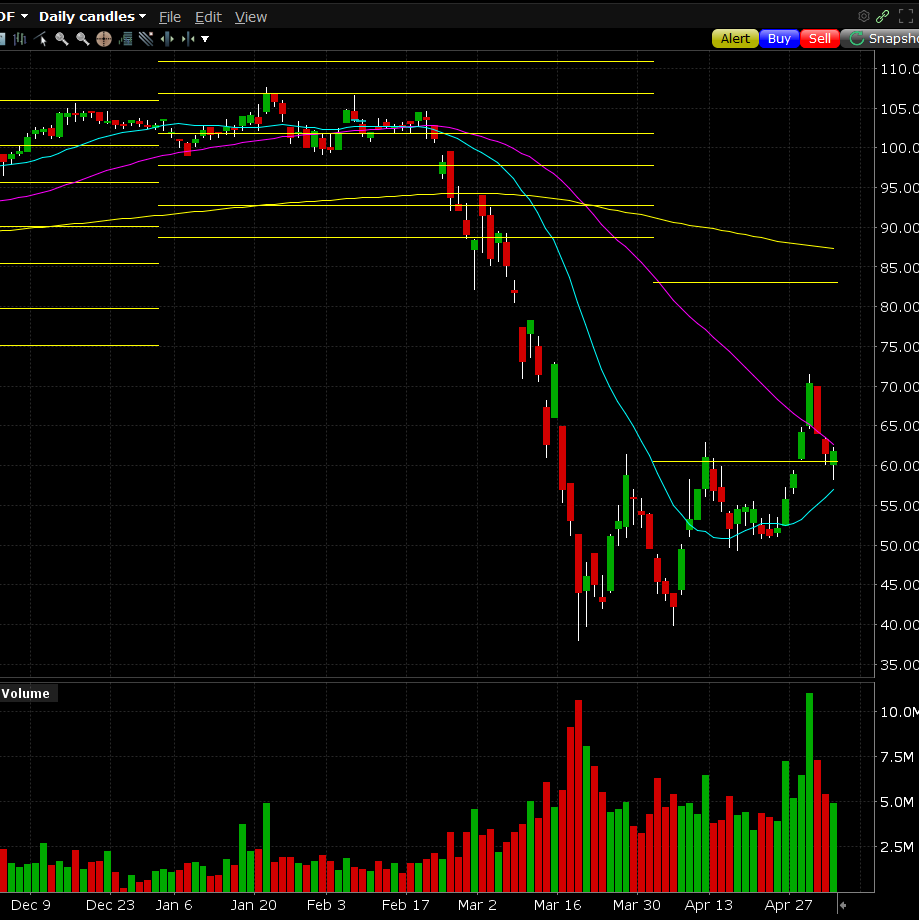
\includegraphics[scale=0.3, height=8.5cm, keepaspectratio]{cropped}
\label{fig:myfig}
\end{wrapfigure}

The purple and blue lines are called the VWAP, the volume-weighted average price. It smooths the last n candles by considering the volume of that candle - note that this information is built directly on top of candle data. The VWAP is one of the most commonly used indicators in big finance, and large hedge funds include it in their decision-making processes. They look for instances when the candles cross the VWAP, and take that as a buy or sell signal (buy if cross upwards, sell if cross downwards).\\
The size of the bars can be adjusted, and the indicators adjust accordingly to factor in the new scale. So it results in indicators that are tightly couple to the refinement, as a thirty minute candlestick chart will keep largely different signals than a five minute chart will.

\section*{1.3 Order Book, linearity, and TDA}

The issue with the form of analysis outlined above, which is the most common form of financial analysis, is that we get indicators that are tightly couple with the data type, and are defined linearly based on the time series data. This is where the advent of topological data analsis (TDA) brings a wealth of information. Furthermore, we shift our attention from the consolidated forms of financial data, to the most granular form of data, which is orderbook data. Orderbook data is not considered time-series, but rather event-driven; the events are new orders entering the market, order executions, or cancellations. All of these update the state of the orderbook. We present below an example of orderbook data; note here the data IS timestamped, which is not the norm, but was necessary to make the computation for this paper permissible. The loss of accuracy is negligible as we timestamp the order by per second
\begin{figure}[h]
\centering
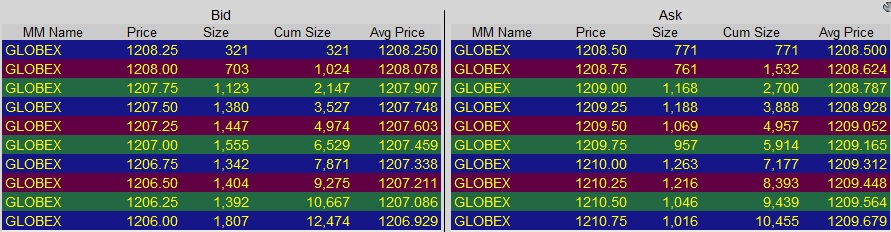
\includegraphics[scale=0.7]{market_depth}
\end{figure}

The orderbook lists all the orders at every price of a stock. For example, 1208.00 has 703 orders, which are by definition buy limit orders. 1209.5 has 1069 order, which are sell limit orders. This method of data is reliant on the participants within the market, as each and every order is listed, and all order events are accounted for. Clearly, this would be massive amounts of data to process, and to find patterns in it would require superb learning models and computational power. This is where we employ TDA to find shape-like structures in the data.\\


\section*{1.4 Summary}

In effect, we aim to eliminate dependency of outcomes on timeframe of the data, and to shift our focus from studying the market as a whole to studying its participants, by using order-book data. We then look for patterns within this data by considering persistence homology and other topological invariants.

\part{Methods of TDA}
The method that we will describe is the use of persistence homology. We embed the orderbook data into some ambient euclidean space, where the dimension is defined by the number of levels in our orderbook. We assume that we look at finite levels. We construct a filtration of simplicial complexes, and order them according to a resolution parameter. As the resolution changes, some features appear in the simplicial complexes while others dissappear. We give each feature a birth and death value, and the difference will represent the persistence of that feature. As can be seen, through this method we do not lose any information, and all topological features are considered; there is no smoothing\cite{gidea2018topological}.\\
We embed our orderbook to get a point cloud data set $X=\{x_1,...,x_n\}$ in $\Reals^d$. For every $\epsilon>0$, we let $R(X,\epsilon)$ be the Vietoris-Rips simplicial complex. If $\epsilon$ is the resolution, and $\epsilon'<\epsilon$, we have $R(X,\epsilon')\subseteq R(X,\epsilon)$. We are interested in the homology groups corresponding to these simplexes. Note that if $\epsilon'<\epsilon$, then $H_k(R(X,\epsilon'))\subseteq H_k(R(X,\epsilon))$, i.e. filtrations carry to all levels of homology groups. The non-zero k-dimensional homology classes $\alpha$ are the features that we study. For each $\alpha$ there are $\eone$ and $\etwo$ such that $\alpha\in H_k(R(X,\epsilon))$ but it is not in the image of any $H_k(R(X,\epsilon-\delta))$ for $\delta>0$, and $H_k(R(X,\epsilon'))$ is non-sero for all $\eone<\epsilon'<\etwo$, but the image of $\alpha$ in $H_k(R(X,\etwo))$ is zero. We say $\alpha$ is born at $b_\alpha = \eone$ and dies at $d_\alpha = \etwo$. The multiplicity $\mu_\alpha(b_\alpha,d_\alpha)$ is the number of $\alpha$ that are born and die at the respective values. This multiplicity exists as we constructed a finite simplicial complex \cite{chazal2017introduction}.\\
We translate the information on the k-dimensional homology generators in a persistence diagram $P_k$ consisting of:
\begin{itemize}
\item
For each $\alpha$ we assign $z_\alpha=(b_\alpha,d_\alpha)\in\Reals^2$ together with $\mu_\alpha(b_\alpha,d_\alpha)$.
\item
$P_k$ consists of all points in the positive diagonal of $\Reals^2$, which are the trivial generators that are born and die instantaneously.
\end{itemize}
% Persistence diagram photo
\begin{wrapfigure}{r}{0.55\linewidth}
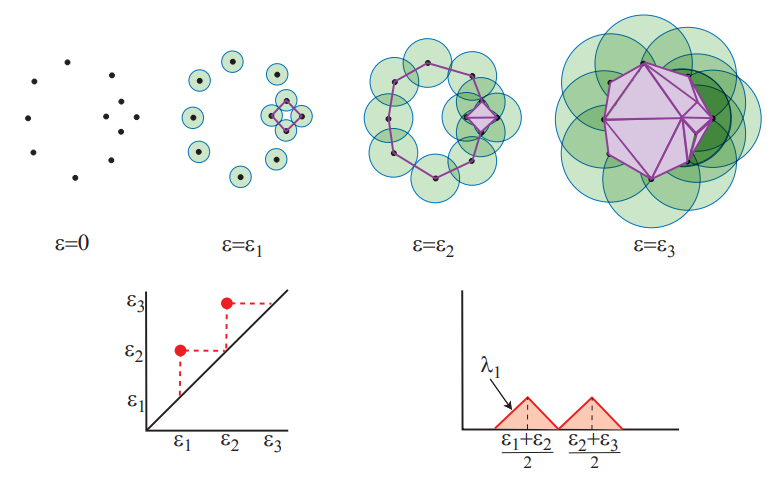
\includegraphics[scale=0.3, height=6.5cm, keepaspectratio]{persistence_diagram}
\end{wrapfigure}

The axes are birth indices on the horizontal, and death indices on the vertical. We will endow this space of persistence diagrams with a metric, namely the degree p Wasserstein distance, for $p\geq 1$, defined by
\begin{equation*}
W_p(P^1_k, P^2_k) = inf_\psi(\sum_{q\in P_k^1}||x-\psi(x)||^p_\infty)^{1/p}
\end{equation*}
where $\psi:P_k^1\to P_k^2$ are bijections, and $||.||_\infty$ is the usual sup norm.\\
In direct contrast to the fragility of indicators in time-series format, persistence homology is greatly robust under perturbation, and thus more suitable for analyzing noisy data, especially orderbook data. That is, the wasserstein distance between persistence diagrams changes in proportion to changes in the underlying data set \cite{chazal2017introduction}.\\
Labelling the space of persistance diagrams as $\mathcal{P}$, we have a metric space $(\mathcal{P},W_p)$. This metric space is not complete, but can be embedded into a function space and inherit this property. 
%Cite here
Once this embedding is done, we can analyze the data using statistical methods. One such form would be to construct a dynamical system on a bundle of order books. Suppose we have a universe of different stock order books $\mathcal{U}$, and at each time t, we have the complete form of the space of persistence diagrams on each stock. We can study the invariance of homology classes across the order books, and the birth and death rates of reoccuring homology classes. Using this information, we can construct correlation matrices indexed by t, and use some learning paradigm to predict the persistence of these same features on out-of-sample data. Furthermore, we can endow the spaces of persistence diagrams with the differentiable structure of the function space, and thus gain a smooth dynamical system. By restricting the systems to spaces of persistence diagrams on each order, we have a k-dimensional distribution, and can possibly gain further insight through frobenius theorem if there exist integral submanifolds.

\part{Conclusion}

Using methods of persistence homology, we are able to construct complete metric spaces and conduct statistical treatment. Furthermore, we can ensue further analysis if the distributions of the persistence diagrams in our stock universe admit integral submanifolds. Using these geometrical and topological methods, we gain robust insight into invariants within the orderbook, and do not lose information due to smoothing. We can construct natural indicators in this manner by considering homology classes that persist for long periods, and are strongly correlated to patterns within the data. This is in contrast to indicators that are normally built on top of candlestick data, which are highly coupled to the data type, non-robust, and sensitive to perturbations. The use of persistence homology allows for anti-fragile trading methods, especially when the space is endowed with a differentiable structure.\\
Future steps would include the study of persistent features when the space is also endowed with a geometry. In this manner we can consider distances between persistence diagrams at different points of our dynamical system, and gain deep insight about the behaviour of markets in anomolous situations, such as financial crashes.
\bibliographystyle{plain}
\nocite{*}
\bibliography{bibliography_327.bib}
\end{document}